%%%%%%%%%%%%%%%%%%%%%%%%%%%%%%%%%%%%%%%%%%%%%%%%%%%%%%%%%%%%%%%%%%
%%%%%%%%%%%%%%%%%%%%%%%%%%%%%%%%%%%%%%%%%%%%%%%%%%%%%%%%%%%%%%%%%%
%Packages
\documentclass[10pt, a4paper]{article}
\usepackage[top=3cm, bottom=4cm, left=3.5cm, right=3.5cm]{geometry}
\usepackage{amsmath,amsthm,amsfonts,amssymb,amscd, fancyhdr, color, comment, graphicx, environ}
\usepackage{float}
\usepackage{mathrsfs}
% \usepackage[math-style=ISO]{unicode-math}
% \setmathfont{TeX Gyre Termes Math}
\usepackage{lastpage}
\usepackage[dvipsnames]{xcolor}
\usepackage[framemethod=TikZ]{mdframed}
\usepackage{enumerate}
\usepackage[shortlabels]{enumitem}
\usepackage{fancyhdr}
\usepackage{indentfirst}
\usepackage{listings}
\usepackage{sectsty}
\usepackage{thmtools}
\usepackage{shadethm}
\usepackage{hyperref}
\usepackage{setspace}
\hypersetup{
    colorlinks=true,
    linkcolor=blue,
    filecolor=magenta,      
    urlcolor=blue,
}

%%%%%%%%%%%%%%%%%%%%%%%%%%%%%%%%%%%%%%%%%%%%%%%%%%%%%%%%%%%%%%%%%%
%                      Added Packages
%%%%%%%%%%%%%%%%%%%%%%%%%%%%%%%%%%%%%%%%%%%%%%%%%%%%%%%%%%%%%%%%%%

\usepackage{siunitx}
\usepackage{caption}
\usepackage[spanish]{babel}
\renewcommand{\spanishtablename}{Tabla}

%%%%%%%%%%%%%%%%%%%%%%%%%%%%%%%%%%%%%%%%%%%%%%%%%%%%%%%%%%%%%%%%%%
%%%%%%%%%%%%%%%%%%%%%%%%%%%%%%%%%%%%%%%%%%%%%%%%%%%%%%%%%%%%%%%%%%
%Environment setup
\mdfsetup{skipabove=\topskip,skipbelow=\topskip}
\newrobustcmd\ExampleText{%
An \textit{inhomogeneous linear} differential equation has the form
\begin{align}
L[v ] = f,
\end{align}
where $L$ is a linear differential operator, $v$ is the dependent
variable, and $f$ is a given non−zero function of the independent
variables alone.
}
\mdfdefinestyle{theoremstyle}{%
linecolor=black,linewidth=1pt,%
frametitlerule=true,%
frametitlebackgroundcolor=gray!20,
innertopmargin=\topskip,
}
\mdtheorem[style=theoremstyle]{Problem}{Problem}
\newenvironment{Solution}{\textbf{Solution.}}

\definecolor{codegreen}{rgb}{0,0.6,0}
\definecolor{codegray}{rgb}{0.5,0.5,0.5}
\definecolor{codepurple}{rgb}{0.58,0,0.82}
\definecolor{backcolour}{rgb}{0.95,0.95,0.92}

\lstdefinestyle{mystyle}{
    backgroundcolor=\color{backcolour},   
    commentstyle=\color{codegreen},
    keywordstyle=\color{magenta},
    numberstyle=\tiny\color{codegray},
    stringstyle=\color{codepurple},
    basicstyle=\ttfamily\footnotesize,
    breakatwhitespace=false,         
    breaklines=true,                 
    captionpos=b,                    
    keepspaces=true,                 
    numbers=left,                    
    numbersep=5pt,                  
    showspaces=false,                
    showstringspaces=false,
    showtabs=false,                  
    tabsize=2
}

\lstset{style=mystyle}
%%%%%%%%%%%%%%%%%%%%%%%%%%%%%%%%%%%%%%%%%%%%%%%%%%%%%%%%%%%%%%%%%%
%%%%%%%%%%%%%%%%%%%%%%%%%%%%%%%%%%%%%%%%%%%%%%%%%%%%%%%%%%%%%%%%%%
%Fill in the appropriate information below
\newcommand{\norm}[1]{\left\lVert#1\right\rVert}     
\newcommand\course{XXXX0000}                            % <-- course name   
\newcommand\hwnumber{0}                                 % <-- homework number
\newcommand\Information{Someone}                        % <-- personal information
%%%%%%%%%%%%%%%%%%%%%%%%%%%%%%%%%%%%%%%%%%%%%%%%%%%%%%%%%%%%%%%%%%
%%%%%%%%%%%%%%%%%%%%%%%%%%%%%%%%%%%%%%%%%%%%%%%%%%%%%%%%%%%%%%%%%%
%Page setup
\pagestyle{fancy}
\headheight 35pt
\lhead{\today}
\rhead{
\includegraphics[width=3cm]{images/logosimbolo-horizontal.png}}
\lfoot{}
\pagenumbering{arabic}
\cfoot{\small\thepage}
\rfoot{}
\headsep 1.2em
\renewcommand{\baselinestretch}{1.25}
%%%%%%%%%%%%%%%%%%%%%%%%%%%%%%%%%%%%%%%%%%%%%%%%%%%%%%%%%%%%%%%%%%
%%%%%%%%%%%%%%%%%%%%%%%%%%%%%%%%%%%%%%%%%%%%%%%%%%%%%%%%%%%%%%%%%%
%Add new commands here
\renewcommand{\labelenumi}{\alph{enumi}}
\newcommand{\Z}{\mathbb Z}
\newcommand{\R}{\mathbb R}
\newcommand{\Q}{\mathbb Q}
\newcommand{\NN}{\mathbb N}
\newcommand{\PP}{\mathbb P}
\DeclareMathOperator{\Mod}{Mod} 
\renewcommand\lstlistingname{Algorithm}
\renewcommand\lstlistlistingname{Algorithms}
\def\lstlistingautorefname{Alg.}
\newtheorem*{theorem}{Theorem}
\newtheorem*{lemma}{Lemma}
\newtheorem{case}{Case}
\newcommand{\assign}{:=}
\newcommand{\infixiff}{\text{ iff }}
\newcommand{\nobracket}{}
\newcommand{\backassign}{=:}
\newcommand{\tmmathbf}[1]{\ensuremath{\boldsymbol{#1}}}
\newcommand{\tmop}[1]{\ensuremath{\operatorname{#1}}}
\newcommand{\tmtextbf}[1]{\text{{\bfseries{#1}}}}
\newcommand{\tmtextit}[1]{\text{{\itshape{#1}}}}

\newenvironment{itemizedot}{\begin{itemize} \renewcommand{\labelitemi}{$\bullet$}\renewcommand{\labelitemii}{$\bullet$}\renewcommand{\labelitemiii}{$\bullet$}\renewcommand{\labelitemiv}{$\bullet$}}{\end{itemize}}
\catcode`\<=\active \def<{
\fontencoding{T1}\selectfont\symbol{60}\fontencoding{\encodingdefault}}
\catcode`\>=\active \def>{
\fontencoding{T1}\selectfont\symbol{62}\fontencoding{\encodingdefault}}
\catcode`\<=\active \def<{
\fontencoding{T1}\selectfont\symbol{60}\fontencoding{\encodingdefault}}

%%%%%%%%%%%%%%%%%%%%%%%%%%%%%%%%%%%%%%%%%%%%%%%%%%%%%%%%%%%%%%%%%%
%%%%%%%%%%%%%%%%%%%%%%%%%%%%%%%%%%%%%%%%%%%%%%%%%%%%%%%%%%%%%%%%%%
%Begin now!



\begin{document}

\begin{titlepage}
    \begin{center}
            
        \huge
        \textbf{Entrega 2: Evaluación de la Enfermedad de Parkinson Mediante Datos de Escritura a Mano}\\
        
        \huge
        Fundamentos de Deep Learning
        
        \vspace{1cm}
        Jeferson Gallo\\
        \large
        jeferson.gallo@udea.edu.co

        \vspace{1cm}
        
        \Large
       Estudiante de Maestía en Ingeniería de Telecomunicaciones\\
        Facultad de Ingeniería, Universidad de Antioquia

        \vspace{1.5cm}
        
        \begin{figure}[h!]
            \centering
            \includegraphics[width=8cm]{images/logosimbolo-vertical.png}
            %\caption{}
            %\label{fig:enter-label}
        \end{figure}
        
        \vfill
        \Large
        \today
            
    \end{center}
\end{titlepage}

%%%%%%%%%%%%%%%%%%%%%%%%%%%%%%%%%%%%%%%%%%%%%%%%%%%%%%%%%%%%%%%%%%
%%%%%%%%%%%%%%%%%%%%%%%%%%%%%%%%%%%%%%%%%%%%%%%%%%%%%%%%%%%%%%%%%%
%Start the assignment now
%%%%%%%%%%%%%%%%%%%%%%%%%%%%%%%%%%%%%%%%%%%%%%%%%%%%%%%%%%%%%%%%%%
%New problem
\newpage

\subsection*{Contexto}

La enfermedad de Parkinson (EP) es una enfermedad neurodegenerativa que afecta 
el sistema nervioso central mediante la pérdida progresiva de neuronas 
dopaminérgicas~\cite{ref1}. La dopamina es un neurotransmisor encargado del 
funcionamiento de las vías neuronales asociadas con la motivación, el estado de 
ánimo y el control motor~\cite{ref2}. Por esta razón, la EP puede causar síntomas 
motores como la bradicinesia (lentitud en los movimientos voluntarios), la rigidez 
muscular y los temblores en reposo. Estos síntomas afectan significativamente 
diferentes actividades de los pacientes como lo es la escritura a mano, ya que los 
procesos de escritura necesitan una alta coordinación de los músculos y tendones 
que conectan el antebrazo, la muñeca y los dedos. Adicionalmente, las principales 
anomalías que se evidencia en la escritura son la micrografía (reducción anormal en 
el tamaño de la escritura) y la disgrafía (déficits en la producción grafomotora 
debido a una combinación de varios signos cardinales de la enfermedad de Parkinson)~\cite{ref32}.


\subsection*{Objetivo de Machine Learning}

En este proyecto se abordará una clasificación bi-clase entre pacientes con la enfermedad de Parkinson 
versus personas sanas (HC) mediante señales de escritura a mano, utilizando diferentes tareas como dibujos, 
escritos y una tarea compleja. Las imágenes correspondientes a cada tarea se procesan mediante una red 
convolucional VGG-16, la cual fue entrenada con la base de datos ImageNet. El objetivo principal se 
basa en determinar cuál de las diferentes tareas de escritura me permite un mejor modelamiento de 
la enfermedad de parkinson.



\subsection*{Datos}

Los datos fueron recopilados utilizando una tableta Wacom Cintiq 13 HD con retroalimentación visual 
para los participantes y con una frecuencia de muestreo de 180 Hz. Esta tableta proporciona seis 
señales diferentes provenientes del proceso de escritura: la posición $x$, la posición $y$, la distancia 
desde la superficie hasta el lápiz (la posición $z$), la presión del lápiz, el ángulo azimut y la 
inclinación del lápiz (la altitud). Para la creación de las imágenes se utilizan las señales $(x,y)$
las cuales corresponden a los trazos realizados sobre la superficie de la tablet. Un ejemplo de las
imágenes resultantes para algunas tareas se encuentran en la Figura~\ref*{fig:db_images}.

Para este trabajo se tienen un total de 7 tareas dentro de las cuales se encuentran algunos escritos 
como el alfabeto, frase libre y nombre; tareas de dibujo como una línea curva, espiral y una casa; y 
finalmente se tiene una tarea compleja llamada rey. En la Tabla~\ref{tab:gita_data} se encuentran 
la cantidad de participantes por cada una de las tareas. 


\begin{figure}
    \centering
    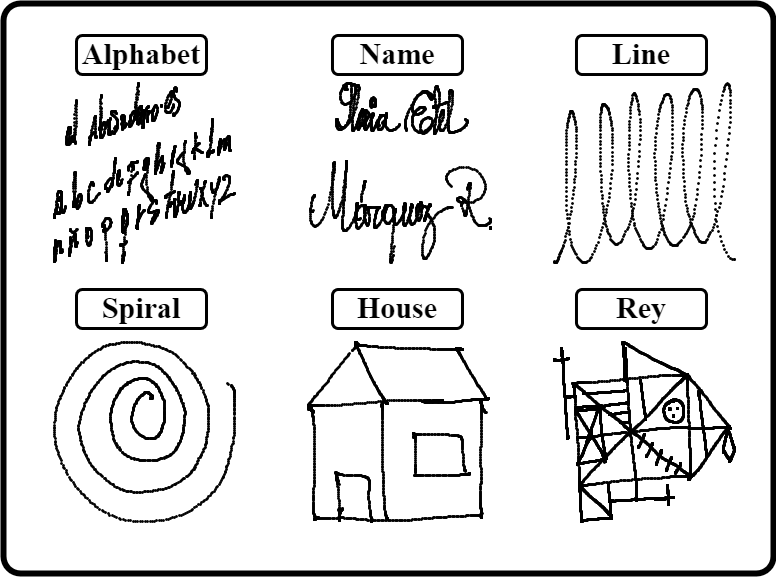
\includegraphics[width=0.6\textwidth]{images/HW_Tasks.png}
    \caption{Imágenes de la base de datos.}
    \label{fig:db_images}
\end{figure}


\begin{table}[h!!]
\caption{Cantidad de participantes entre pacientes (PD), y controles (HC), en cada una de las tareas.}
\centering
\label{tab:gita_data}
%\resizebox{\linewidth}{!}{
\begin{tabular}{ccc}
\hline
\textbf{Tarea}       & \textbf{\# Pacientes (PD)} & \textbf{\# Controles (HC)} \\ \hline
\textbf{alphabet}    & 71                         & 55                         \\
\textbf{line1}       & 60                         & 42                         \\
\textbf{freewriting} & 73                         & 54                         \\
\textbf{house}       & 75                         & 55                         \\
\textbf{rey}         & 69                         & 54                         \\
\textbf{name}        & 74                         & 55                         \\
\textbf{spiral}      & 75                         & 55                         \\ \hline
\end{tabular}
%}
\end{table}


\subsection*{Metricas de desempeño}

En este proyecto se utilizarán métricas como la matriz de confusión, como también algunas 
métricas que se desprenden de esta. 

\subsubsection*{Matriz de confusión}

Es una matriz cuadrada donde el número de filas y columnas depende de la cantidad de clases 
diferentes que tenga el problema. Esta matriz organiza las predicciones correctas e incorrectas 
evidenciando el rendimiento del sistema para la predicción de cada clase. En problemas de 
clasificación bi-clase, la matriz de confusión es $2 \times 2$ donde en cada celda se pueden 
definir los siguientes términos:

\begin{itemize}
    \item \textit{Verdaderos positivos (TP, true positive):} es la cantidad de datos de la clase positiva que el sistema clasifico correctamente.

    \item \textit{Falsos positivos (FP, false positive):} son la cantidad de datos de la clase positiva que el sistema clasifico erróneamente como pertenecientes a la clase negativa.

    \item \textit{Verdaderos negativos (TN, true negative):} es el número de datos de la clase negativa clasificados correctamente por el sistema.

    \item \textit{Falsos negativos (FN, false negative):} es el número de datos de la clase negativa que el sistema clasifico erróneamente como pertenecientes a la clase positiva.
    
\end{itemize}

Además, otras métricas pueden ser estimadas de acuerdo con la información de la matriz de confusión:

\begin{itemize}
    \item \textit{Exactitud (acc, accuracy):} se define como la cantidad de aciertos en ambas clases sobre el total de datos.

    \begin{equation}
        acc = \frac{TP + TN}{TP + FP + TN + FN}
    \end{equation}

    \item \textit{Sensibilidad (S, sensitivity):} es la capacidad del sistema para clasificar la clase positiva.
    
    \begin{equation}
        S = \frac{TP}{TP+FN}
    \end{equation}

    \item \textit{Especificidad (E, especificity):} es la capacidad del sistema para clasificar la clase negativa.
    
    \begin{equation}
        E = \frac{TN}{TN+FP}
    \end{equation}

    \item \textit{Precisión (P, precision):} mide la proporción de muestras positivas predichas correctamente entre todas las muestras que se predicen como positivas.

    \begin{equation}
        P = \frac{TP}{TP+FP}
    \end{equation}

    \item \textit{F1-socre:} es la media armónica entre la precisión y la sensibilidad, la cual permite obtener una medición balanceada del desempeño del modelo.

    \begin{equation}
        F1-score = 2 \times \frac{P \times S}{P+S}
    \end{equation}
    
\end{itemize}

\subsection*{Modelo de Deep Learning}

\begin{figure}[h!!]
    \centering
    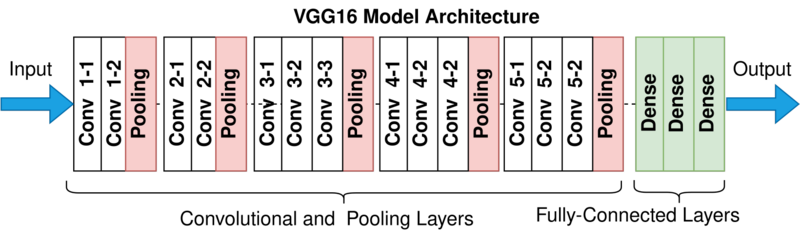
\includegraphics[width=1\textwidth]{images/VGG16.png}
    \caption{Arquitectura VGG16.}
    \label{fig:vgg}
\end{figure}


Para este trabajo se implementó la red neuronal convolucional VGG16. Esta es una arquitectura 
desarrollada por el Visual Geometry Group (VGG) de la Universidad de Oxford, que se destacó 
en la competición ImageNet Large Scale Visual Recognition Challenge (ILSVRC) de 2014. Se 
caracteriza por su simplicidad y efectividad, utilizando principalmente pequeñas capas 
convolucionales de 3$\times$3 píxeles y capas de max-pooling de 2$\times$2 píxeles, organizadas en 5 bloques 
de capas convolucionales. Esta arquitectura ha demostrado ser 
extremadamente eficiente en tareas de reconocimiento de imágenes, estableciendo un nuevo 
estándar en precisión y eficiencia en el campo del aprendizaje profundo~\cite{ref9}. El modelo 
implementado en este trabajo~\ref*{fig:vgg} fue pre-entrenado con la base de datos ImageNet y se le agregan
dos capas densas para realizar la clasificación entre pacientes y controles. 


\subsection*{Experimentos}

\subsubsection*{Exploración de tareas}

Para este primer experimento se desea conocer cuál de las tareas utilizadas modela de una mejor manera
la enfermedad del parkinson en la tarea de clasificación. En la Tabla~\ref*{tab:VGG16_Freeze} se encuentran
los resultados obtenidos para las tareas cuando no se afinan ningún bloque convolucional y solamente se afinan
las capas densas encargadas de realizar la clasificación. En la Tabla~\ref*{tab:VGG16_tuned} se encuentran 
los resultados del experimento cuando se afinan todos los bloques convolucionales y las capas densas de la red.
En ambos casos la tarea de escritura del nombre obtuvo exactitudes del 84\% del modelo sin afinar y 73.08\%
cuando se afinaron todos los bloques convolucionales.


\begin{table}[h!!]
\caption{Resultados de la exploración de tareas utilizando el modelo VGG16 sin afinar.}
\centering
\label{tab:VGG16_Freeze}
%\resizebox{\linewidth}{!}{
\begin{tabular}{ccccc}
\hline
\textbf{Task}        & \textbf{Accuracy} & \textbf{Specificity} & \textbf{Sensitivity} & \textbf{F1\_Score} \\ \hline
\textbf{name}        & 84.62             & 100.00               & 75.00                & 0.86               \\
\textbf{spiral}      & 76.92             & 86.67                & 63.64                & 0.70               \\
\textbf{rey}         & 76.00             & 63.64                & 85.71                & 0.80               \\
\textbf{alphabet}    & 65.38             & 54.55                & 73.33                & 0.71               \\
\textbf{house}       & 57.69             & 41.67                & 71.43                & 0.65               \\
\textbf{line1}       & 42.86             & 37.50                & 46.15                & 0.50               \\
\textbf{freewriting} & 23.08             & 23.08                & 23.08                & 0.23               \\ \hline
\end{tabular}
%}
\end{table}



\begin{table}[h!!]
\caption{Resultados de la exploración de tareas afinando todos los bloques convolucionales 
del modelo VGG16.}
\centering
\label{tab:VGG16_tuned}
%\resizebox{\linewidth}{!}{
\begin{tabular}{ccccc}
\hline
\textbf{Task}        & \textbf{Accuracy} & \textbf{Specificity} & \textbf{Sensitivity} & \textbf{F1\_Score} \\ \hline
\textbf{name}        & 73.08             & 70.00                & 75.00                & 0.77               \\
\textbf{spiral}      & 73.08             & 66.67                & 81.82                & 0.72               \\
\textbf{alphabet}    & 65.38             & 72.73                & 60.00                & 0.67               \\
\textbf{rey}         & 64.00             & 54.55                & 71.43                & 0.69               \\
\textbf{house}       & 57.69             & 58.33                & 57.14                & 0.59               \\
\textbf{freewriting} & 53.85             & 53.85                & 53.85                & 0.54               \\
\textbf{line1}       & 47.62             & 37.50                & 53.85                & 0.56               \\ \hline
\end{tabular}
%}
\end{table}

\subsubsection*{Exploración de la tare "Name"}

Debido a que en el anterior experimento la tarea name obtuvo el mejor desempeño en ambos casos, además
se observó una variación entre el uso del modelo sin afinar y afinando todas las capas. En este experimento
se exploran diferentes grados de afinación de los bloques convolucionales. En la Tabla~\ref*{tab:VGG16_block}
se observan los resultados al variar la cantidad de bloques convolucionales afinados. El mejor resultado 
finalmente fue afinando solamente la capa densa que corresponde a la etapa de clasificación. Esto puede estar 
ocurriendo debido a la poca cantidad de datos, ya que no se alcanzan a afinar correctamente todas las capas
convolucionales para modelar el fenómeno del parkinson.

\begin{table}[h!!]
\caption{Resultados de la exploración de tareas afinando todos los bloques convolucionales 
del modelo VGG16.}
\centering
\label{tab:VGG16_block}
\resizebox{\linewidth}{!}{
\begin{tabular}{ccccccc}
\hline
\textbf{Block}  & \textbf{Total parameters} & \textbf{Trainable parameters} & \textbf{Accuracy} & \textbf{Specificity} & \textbf{Sensitivity} & \textbf{F1\_Score} \\ \hline
\textbf{dense}  & 14,780,610                & 65,922                        & 87.50             & 100.00               & 75.00                & 0.86               \\
\textbf{block5} & 14,780,610                & 7,145,346                     & 73.08             & 100.00               & 56.25                & 0.72               \\
\textbf{block4} & 14,780,610                & 13,045,122                    & 53.85             & 60.00                & 50.00                & 0.57               \\
\textbf{block3} & 14,780,610                & 14,520,450                    & 65.38             & 100.00               & 43.75                & 0.61               \\
\textbf{block2} & 14,780,610                & 14,741,890                    & 76.92             & 100.00               & 62.50                & 0.77               \\
\textbf{block1} & 14,780,610                & 14,780,610                    & 73.08             & 70.00                & 75.00                & 0.77               \\ \hline
\end{tabular}
}
\end{table}


\section*{Análisis de resultados}
En la Figura~\ref*{fig:History} se encuentra el proceso de entrenamiento del mejor experimento el
cual corresponde a la tarea "name" cuando solo se afina la capa densa. Se configuró un total de 2000
épocas con una paciencia para el early stopping de 100. En total fueron necesarias 1400 épocas para
afinar el modelo. Adicionalmente, en la Figura~\ref*{fig:cm} se encuentra la matriz obtenida para el
conjunto de test en este experimento. En este caso, el 100\% de los controles fué clasificado correctamente
mientras que el 75\% de los pacientes pudieron ser identificados por el modelo.

\begin{figure}[h!!]
    \centering
    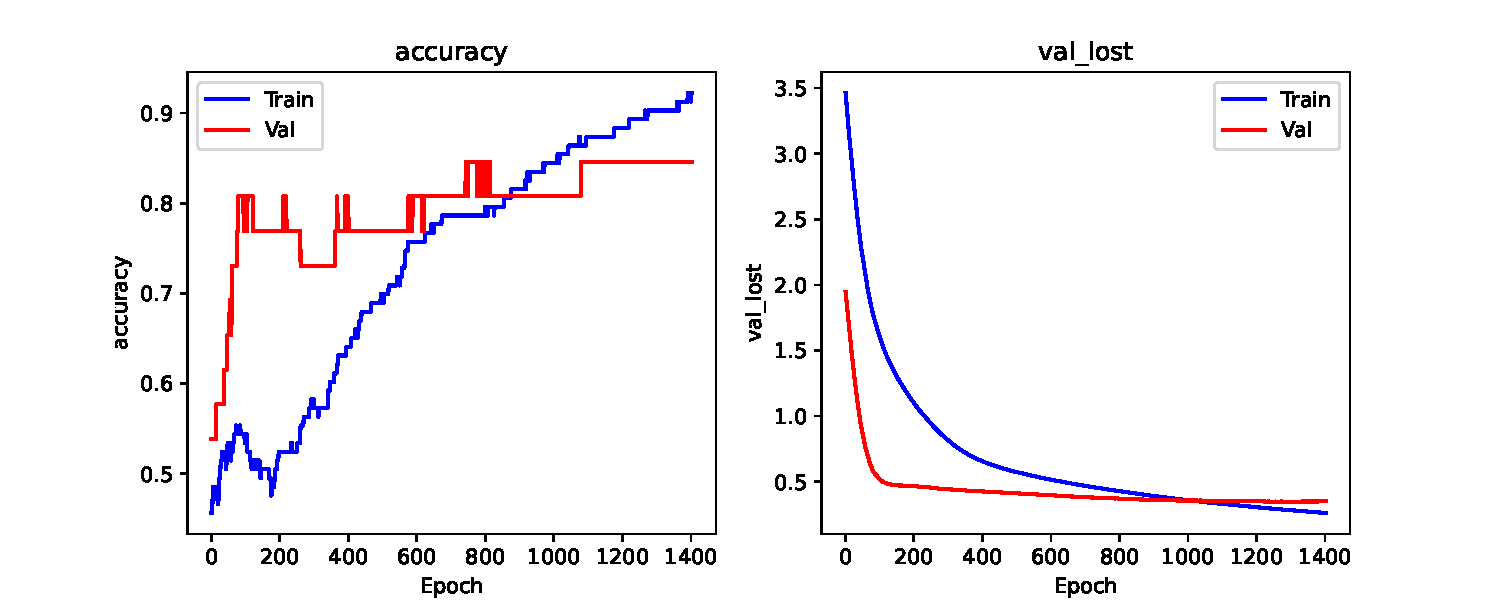
\includegraphics[width=1\textwidth]{images/History_Name_Dense.pdf}
    \caption{Curvas de entrenamiento en la tarea "name" afinando las capas densas.}
    \label{fig:History}
\end{figure}

\begin{figure}[h!!]
    \centering
    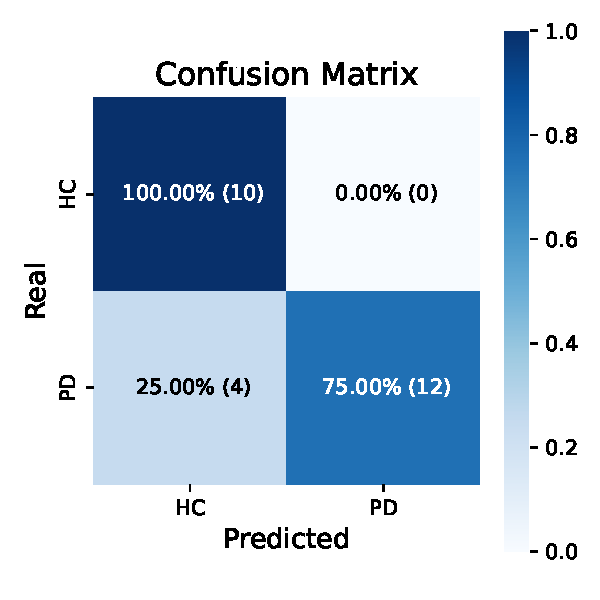
\includegraphics[width=0.6\textwidth]{images/CM_Name_Dense.pdf}
    \caption{Matiz de confusión para el experimento del nombre cuando se afinan las capas densas.}
    \label{fig:cm}
\end{figure}


\section*{Discribución de los notebooks}
En el notebook \textbf{1\_Data\_Exploration} se encuentra una breve exploración de la base de
datos, donde se realiza el conteo de participantes por tarea y la visualización de algunas tareas.
En el notebook \textbf{2\_CNN\_Model.ipynb} se encuentra la implementación del
pipeline de entrenamiento. Respecto al script \textbf{3\_Task\_Exploration\_VGG16.py} se realiza el primer
experimento donde se exploran las diferentes tareas. Finalmente, en el script 
\textbf{4\_Name\_CNN\_Models.py} se realizan los experimentos aplicando diferentes niveles de afinación
para la mejor tarea obtenida en el experimento anterior.



\bibliographystyle{splncs04}
\bibliography{refs}

\end{document}

%%%%%%%%%%%%%%%%%%%%%%%%%%%%%%%%%%%%%%%%%%%%%%%%%%%%%%%%%%%%%%%%%%
%%%%%%%%%%%%%%%%%%%%%%%%%%%%%%%%%%%%%%%%%%%%%%%%%%%%%%%%%%%%%%%%%%
